 % \documentclass[a4paper, draft]{report}
\documentclass[a4paper, 10pt]{report}


\usepackage[utf8]{inputenc}
\usepackage[T1]{fontenc}
\usepackage[margin=2.5cm]{geometry}
\usepackage{csquotes}
\usepackage{hyphenat}
\usepackage{biblatex}
\usepackage{graphicx}
\usepackage{float}
\usepackage{caption}
\usepackage{subfig}
\usepackage{textcomp}
\usepackage{gensymb}
\usepackage{booktabs}
\PassOptionsToPackage{hyphens}{url}\usepackage{hyperref}
\usepackage{listings}
\usepackage{lmodern}
\usepackage{amsmath}
\usepackage{amssymb}
\usepackage{siunitx}
\usepackage{enumitem}
\usepackage[acronym]{glossaries}

% \usepackage[scale=1.0]{draftwatermark}

\addbibresource{biblio.bib}
\newacronym{ad}{AD}{Algorithmic/Automatic Differentiation}
\newacronym{sa}{SA}{Spalart Allmaras}
\newacronym{imes}{IMES}{Institute for mechanical systems}

\graphicspath{
    {img}
    {fundamentals/img}
}
% \hyphenation{Mathe-matik wieder-gewinnen}




\title{Extension of the SA turbulence model for rough walls in ADflow}
\author{David Anderegg}

% Add Numbering to chapters
\makeatletter
\def\@makechapterhead#1{%
  \vspace*{50\p@}%
  {\parindent \z@ \raggedright \normalfont
    \interlinepenalty\@M
    \Huge\bfseries  \thechapter.\quad #1\par\nobreak
    \vskip 40\p@
  }}
\makeatother

\renewcommand{\arraystretch}{1.1}



\usepackage{fancyhdr}
\setlength{\headheight}{34pt}

\renewcommand{\headrulewidth}{0.5pt}
\renewcommand{\footrulewidth}{0.5pt}


\fancypagestyle{plain}{
    % header inputs
    \lhead{IMES}
    \chead{Extension of the SA turbulence model for rough walls in ADflow}
    \rhead{
\includegraphics[width=1cm]{uni_header}}


    %footer inputs
    % \lfoot{Innosuisse 35172.1 IP-ENG}
    \cfoot{Page  \thepage}
    \rfoot{\today}
}
\pagestyle{plain}

\setlength{\parskip}{.25em}

\begin{document}
    % \maketitle

    % \begin{abstract}
    %   blablbalabl
    % \end{abstract}

    % \tableofcontents\clearpage
    % \listoffigures\clearpage
    % \listoftables\clearpage


    \chapter{Introduction}
    When performing optimizations, the optimizer tries to maximize the objective as
much as possible. This means, one operates in the limit of the modeling process
used. Imagine an airfoil optimization where the goal is to increase the maximum
coefficient of lift $c_{l}$. In this example, only one design variable is
available: the angle of attack $\alpha$. To simulate the airfoils performance, a
Reynolds Averaged Navier Stokes (RANS) approach is implemented. During the
optimization, the optimizer increases $\alpha$ right until the point where the
flow starts to separate as this is the point where the highest $C_{l}$ lies for
an airfoil. But this means, it is absolutely necessary to accurately predict the
point of separation. When this is not the case, the optimizer exploits effects
that do not exist in reality and thus the whole optimization can not achieve its
full potential. In the worst case, the results obtained might not even be
usable.

ADflow is an open source RANS solver that also computes the gradients of the
objective (and constraints) with respect to the design variables in an efficient
manner called the \textit{adjoint method}. In real life aerodynamic applications,
as airplanes or wind turbines, surface contamination plays an important role.
The primary effect of such contamination is a roughening of the surface. Thus it
is important to be able to simulate and optimize taking the effect of rough
surfaces into account.

\section{Goals}
The goal of this work is to be able to simulate and optimize under the effects
of rough surfaces. ADflow's primary turbulence model is known as \textit{Spalart
  Allmaras}
(SA). It is a one-equation model that was proposed in 1992. It is
widely used for external aerodynamic applications. In 2002, a modification for
rough surfaces was published. This project implements this modification. Thus
the projects aims may be listed as follows:

\begin{itemize}
  \item Modify the existing SA turbulence model for rough walls
  \item Test and verify the implementation.
  \item Use \gls{ad} to differentiate the newly added code. This is needed for
the adjoint method.
  \item Test and verify the modified gradients.
\end{itemize}


\section{ADflow}
Before heading straight in, a few words about ADflow and its history are
provided. It is an open-source RANS solver that is developed and maintained at
\textit{MDOLab} at the university of Michigan. It is based on a structured,
multiblock solver called
\textit{sumb} and has been adapted for gradient based optimization by means of
\textit{Algorithmic Differentiation}\footnote{Thats what AD stands for in
ADflow.} and the \textit{adjoint method}.

In optimization, a lot of simulations are necessary until an optimal design is
found. It is also highly important to always get an objective value for each
design, even if, or especially when, it is unphysical. Otherwise the optimizer
does not know how bad the current design is. To cater those concerns, ADflow
employs some highly efficient and robust NK\footnote{NK stands for the
Newton–Krylov method.} and ANK\footnote{ANK is an approximated Newton–Krylov
method.} solvers. Those can achieve machine-precision convergence, even for
aircraft configurations at an angle of attack of 90\degree
\cite{Mader2020a} \cite{Kenway2019a} \cite{Yildirim2019b}.


Most of ADflow is written in Fortran. But it is interfaced in Python. This means,
the heavy lifting is done in a fast language, but the regular user has the
benefits of an object-oriented high level interpreter language.

\section{Code contributions}
Part of this project is a code contribution to ADflow and a setup of test cases,
both can be found on GitHub under those links:\\


\begin{tabular}{l l}
  ADflow Pull Request & \url{https://github.com/mdolab/adflow/pull/259} \\
  Test cases & \url{https://github.com/DavidAnderegg/SA_rough_testcases}
\end{tabular}


    \chapter{Theoretical Fundamentals}
    \section{Boundary layer}

\subsection{Concept}


\subsection{Turbulent boundary layers}


\subsection{Turbulent boundary layer over rough walls}


\section{Turbulence Models}


\subsection{Spalart Allmaras (SA)}


\subsection{Modification of SA for rough walls}


    \chapter{Methods}
    \section{Implementation}
Before explaining how the modifications for SA-rough were implemented, a couple
of words about the architecture of ADflow are needed.

\paragraph{Block architecture}
This solver only reads \textit{structured grids}, this means all state and grid
variables can be represented in a ``three dimensional table''. One can also think
of a 3d array. This organization is called the \textit{block architecture}. The
index of the block variables are \texttt{i}, \texttt{j} and \texttt{k} for the
x, y and z directions respectively.

\paragraph{Boundary Conditions}
ADflow saves the values of the boundary conditions in a similar way as the block
variables. But they are 2d arrays where the indexes \texttt{i} and \texttt{j}
are used. It is possible to directly relate a volume cell in the block to a
surface cell at the boundary, but it is important to realise surface and volume
cells are different entities.

\paragraph{Global Cell ID}
ADflow assigns a \textit{global cell id} (\texttt{gID} to each volume cell. The
index is an continuously increasing integer that starts at \textbf{0}. It is
applied in a systematic manner that will not be explained further.

\paragraph{Block splitting}
ADflow is capable of solving the governing equations by parallel means. To make
this possible, the whole mesh is split in different blocks. Each processor then
only loads its corresponding block. It is important to realize that no single
processor has access to the whole volume or surface cells\footnote{Assuming more
than one processor is used}.

\subsection{General thoughts}
This modifications requires a little bit more RAM and cpu power. It could also
obscure the standard implementation of the SA model. To cater those
considerations, an on/off switch has been introduced in the python layer called
\texttt{useRoughSA}. When it is \texttt{False}, all implemented changes are
disabled and ADflow behaves exactly as it did before.


\subsection{Changes to wall distance}
The regular SA model needs the distance to the nearest wall. ADflow computes
this distance in a preprocessing step and saves it as a block variable
\texttt{d2wall} for further use. It is slightly more complicated as ADflow can
handle warping meshes and thus this distance needs to be adjusted after each
warp, but this will be explained in more detail later. As shown in equation
\ref{eq:d_new}, the distance to the nearest wall needs to be modified. There are
two strategies to achieve this:

\begin{enumerate}
  \item Overwrite the current \texttt{d2wall} with the modified value. E.g. do
        the modification in a preprocessing step.
  \item Keep the current \texttt{d2wall} as it is and apply the modification
        later when the distance is actually needed.
\end{enumerate}

\noindent Strategy (2) has been chosen as changing the \texttt{d2wall} might
have unforeseen consequences and is just obscuring. But this means, a new block
variable \texttt{ks} needs to be introduced. It will hold the roughness value of
the nearest surface.

\subsubsection{Calculating the distance to the nearest wall}
To be able to assign the correct roughness value of the nearest wall, one must
know which wall is nearest to the current volume cell. For the calculation of
the wall distance, this information is already needed. Thus it was natural to
adapt this function. To explain the changes, one must know how it works:

\begin{enumerate}
  \item The function \texttt{buildClusterWalls} is called. It figures out which
surface mesh belongs to the \textit{no-slip wall} type and gathers all of it on
each processor. This does not scale. But it is assumed the surface mesh is
orders of magnitudes smaller than the volume mesh.  Thus this only becomes a
problem when the size of the volume mesh approaches hundreds of millions of
cells.

Once it has this information, it builds up the whole surface mesh. This is not
straight forward as it might be an overset\footnote{This is also know as Chimera
patch.} mesh where different meshes are overlapping. Therefore it must decide
which cells to drop and which to keep.

After that, it relates the surface mesh to the volume cells and returns the
\texttt{gID}. At first glance, it might seem weird to return ``volume cells''
when the distance to a surface cell is required. But the grid points of both
types are the same and for the walldistance computation the boundary conditions
do not matter.

  \item Once the \texttt{clusterWalls} are built, the function
\texttt{determineWallAssociation} iterates through all the volume cells on the
current processor and figures out which \texttt{gID} of the
\texttt{clusterWalls} is nearest.

Whit that information, it creates a ``PETSc scatter''\footnote{PETSc stands for
Portable, Extensible Toolkit for Scientific Computation.} object called
\texttt{wallScatter}. This object is (in simplified terms) a two dimensional
list which keeps track of which surface cell is nearest to which volume cell. As
the surface cells have been replaced with volume cells before, this is basically
a mapping of volume cells to volume cells.

After that, the memory for \texttt{clusterWalls} is released.

\item A new block variable \texttt{xSurf} is introduced. It holds all the
surface grid points, which are needed for the wall distance calculation for the
volume cells of the current processor. It is the receiving end of the
\texttt{wallScatter} object.

\item In the End, \texttt{updateWallDistancesQuickly} is called to actually
compute the distance to the nearest wall based on the grid points stored in
\texttt{xSurf}.

\item After the mesh has been warped, only \texttt{updateWallDistancesQuickly}
is called. This means, it is assumed the nearest surface cell does not
change, only its coordinates.
\end{enumerate}

\noindent Please note the outlined steps above are in reality a bit more
complicated and only the broad context is described.


\subsubsection{Assigning the block variable \texttt{ks}}
\label{subsubsec:propagate_ks}
To fill the block variable \texttt{ks} with the roughness value of the nearest
surface, the before described walldistance computation is hijacked as follows:

\begin{enumerate}[label=\Alph*]
  \item Introduce a new block variable called \texttt{nearestWallCellInd}. It
holds the \texttt{gID} of the nearest surface cell. Its value is assigned in
step (2) where the \texttt{gID} of the nearest surface cell is determined.

  \item Create a new subroutine called \texttt{updateWallRoughness}. A separate
subroutine is needed as the roughness value on the boundary is only read from
the CGNS\footnote{CGNS stands for CFD General Notation System and is a format
for meshes and their solutions. It is the primary format that ADflow interacts
with.} file once the walldistance has already been calculated. Thus it is not
possible to do it when step (2) is done. ADflow has some helper functions that
allows to overwrite the values of the boundary conditions which are saved in the
CGNS file. Having a separate subroutine to assign \texttt{ks} allows to also use
those helper functions for the wall roughness.
\end{enumerate}

\noindent Now, the inner workings of \texttt{updateWallRoughness} are explained
in more detail:

\begin{enumerate}[label=\Alph*]
  \item Each processor creates two lists: (a) the roughness values of the
surface cells on current processor and (b) the corresponding \texttt{gID}.

  \item Then those two lists are gathered on all processors. This means, every
processor has a list ($\alpha$) of all surface roughness values and ($\beta$) of
all corresponding \texttt{gID}. This does also not scale. But this constraint
has been violated before (in \texttt{buildClusterWalls}) and thus the totally
required RAM is not increased significantly.

\item Now, each processor iterates through its volume cells and requests the
\texttt{gID} from \texttt{nearestWallCellInd}. Then it searches list ($\beta$)
until it finds the same \texttt{gID} and writes down the index \texttt{I} where
it found it.

\item Finally, it assigns the value of list ($\alpha$) at index \texttt{I} to the
block variable \texttt{ks}.
\end{enumerate}

\noindent It is important to note that this strategy can handle different
roughness values for the surface. But those values are not interpolated and are
thus only accurate in the limiting sense of an infinitely fine grid. It can also
lead to weird situations where one single volume cell is assigned a roughness
value where as its surrounding cells are not. This happens because its center is
somehow closest to a small corner of a rough surface cell. This also vanishes
with increasing cell count.

\subsection{SA source terms}
As described in section \ref{subsec:mod_sa_rough}, the terms $\chi$ (equation
\ref{eq:chi_new}) and $f_{v2}$ (equation \ref{eq:fv2_new}) need to be modified.
This has been straight forward. But it is important to not forget the
calculation of $d_{new}$ (equation \ref{eq:d_new}) as this has been postponed in
the previous section.

ADflow employs some Newton-type solvers that require the Jacobian of the
resiudals. Thus it was necessary to also modify the derivative of
$\partial f_{v2} / \partial \tilde \nu$ as follows:

\begin{equation}
  \frac{\partial f_{v2}}{\partial \tilde \nu} =
  \frac{\tilde \nu^{2} \frac{\partial f_{v1}}{\partial \tilde \nu} - \nu}
  {(\tilde \nu f_{v1} + \nu)^{2}}
\end{equation}

\noindent As said before, those changes are only active when \texttt{useRoughSA}
is \texttt{True}.

\subsection{SA boundary conditions}
ADflow employs the concept of \textit{halo cells}. This is an idea to exchange
the boundaries of the split blocks when running in parallel. Take a look at
figure \ref{fig:halo_cells}. On the left side, a block split in 4 is shown. Each
sub-block lives on a different processor. On the right, one can see the
artificial halo cells. After each iteration of the flow solver, the values of
the halo cells are updated with their corresponding values of the other blocks
(red arrows).

\begin{figure}[H] \centering
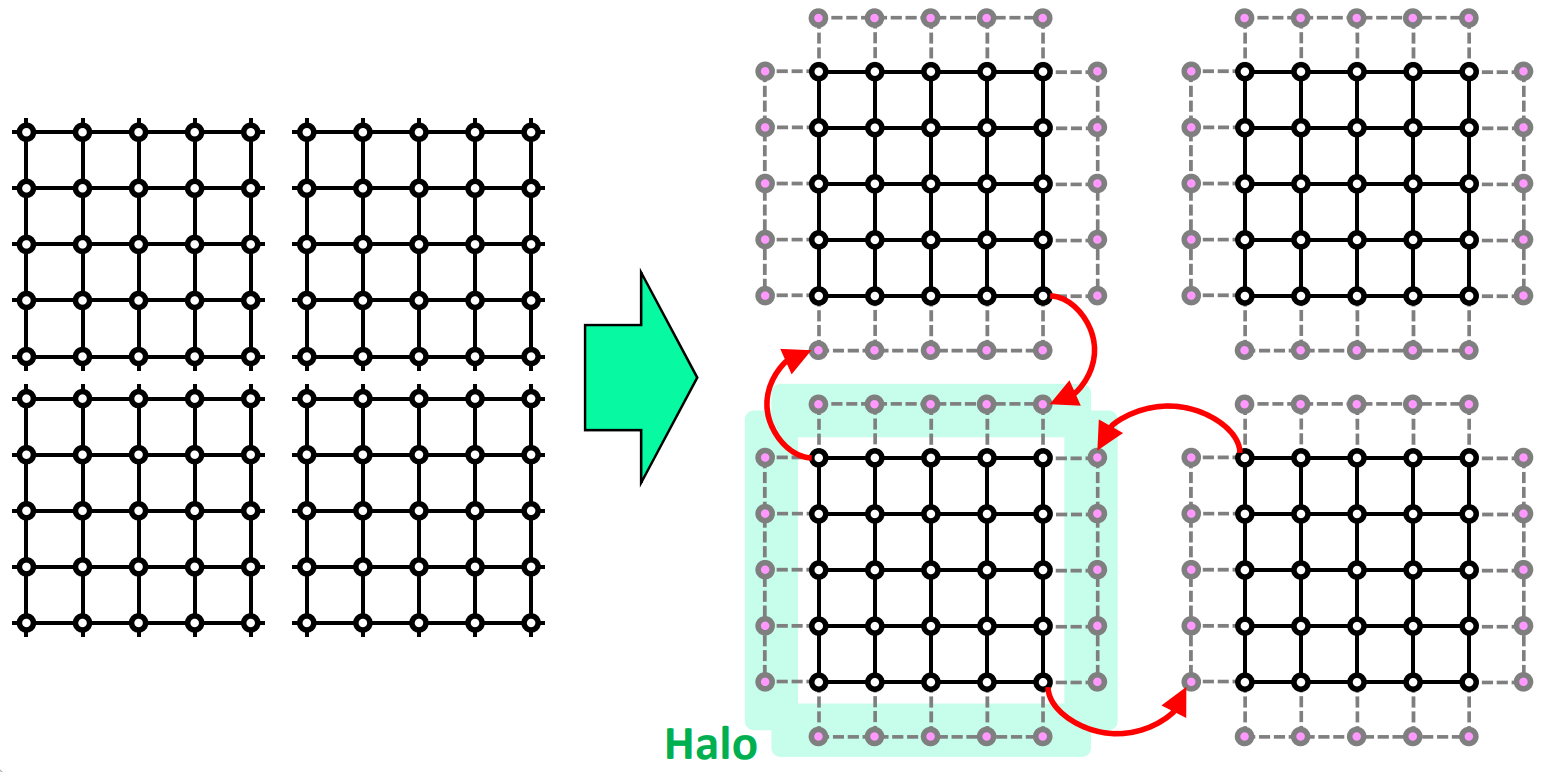
\includegraphics[width=0.7\textwidth]{halo_cells}
    \caption{A block split in 4 (left) and its corresponding halo cells (right)
            \cite{cfd_halo}.}
    \label{fig:halo_cells}
\end{figure}

ADflow is capable of deploying second order schemes and thus needs two layers of
halo cells. But the idea remains the same. As they are not always active, ADflow
takes care of interpolating them by itself.

\paragraph{Explicit boundary conditions}
The concept of halo cells can also be used to prescribe the regular boundary
conditions like a \textit{no-slip wall}. According to equation
\ref{eq:sa_nu_wall_0}, the regular SA model needs a boundary condition of
$\tilde \nu_{wall} = 0$. This means, the first halo is simply updated with the
negative value of the first cell:

\begin{equation}
  \tilde \nu_{h} = - \tilde \nu_{1} \qquad \rightarrow \qquad
  \tilde \nu_{wall} = \frac{\tilde \nu_{1} + \tilde \nu_{h}}{2} = 0
  \label{eq:bc_halo}
\end{equation}

\noindent Where $\tilde \nu_{1}$ is the value of the first interior cell and
$\tilde \nu_{h}$ is the halo cell.

For the rough version, the boundary condition needs to be modified according to
equation \ref{eq:bc_new}:

\begin{equation}
  \left( \frac{\partial \tilde \nu}{\partial n} \right) \equiv
  \frac{\tilde \nu_{1} - \tilde \nu_{h}}{d} =
  \frac{\tilde \nu_{wall}}{0.03 k_{s}}
\end{equation}

\noindent Replacing $\tilde \nu_{wall}$ with equation \ref{eq:bc_halo} and
solving for $\tilde \nu_{h}$, one gets:

\begin{equation}
  \tilde \nu_{h} = \tilde \nu_{1} \frac{0.06 k_{s} - d}{0.06 k_{s} + d}
\end{equation}

\noindent The underlying assumption is, that the first cell to the wall is not
skewed and its center is normal to the wall. But this is in general good practice
and highly recommended for RANS meshes.


\paragraph{Implicit boundary conditions}
ADflow also has some implicit solvers, thus the implicit boundary conditions need to be changed.

TBD!!!!

\subsection{Automatic Differentiation}
As described in \cite{cm1}, ADflow uses Automatic/Algorithmic Differentiation to
compute the partial derivatives which are needed in the \textit{adjoint method}
to compute the total derivatives of the functions of interest with respect to
the design variables. The AD tool used is called \textit{tapenade}
\cite{tapenade}. It is based on JAVA and directly differentiates Fortran source
code. One provides the source code of a Fortran routine, defines the dependent
output variable and the independent input variable with respect to which the
derivative is requested. Tapenade then returns Fortran source code that
computes this derivative.

When the AD architecture for ADflow was set up, tapenade could not handle
parallelization calls using the MPI\footnote{MPI stands for Message Passing
Interface and handles the communication across different processors and
computers when performing parallel computations.}. Thus the decision was made to
split the whole AD in two parts: part (1) communicates data across different
processors, i.e takes care of the parallelization; and part (2) does the actual
computation. This allows tapenade to differentiate the math heavy part (2) and
necessitates the developer to make sure the differentiated routines are called
appropriately (1).


\section{Verification}
The verification of the SA changes is split into two parts: making sure the
roughness values are propagated correctly into the volume cells and verifying SA
rough does actually behave like a rough wall.

\subsection{Roughness propagation}
\label{subsec:roughness_prop}
When assigning a roughness value to the surface, this value gets propagated to
the volume cells as described in section \ref{subsubsec:propagate_ks}. This has
to be tested, especially when running on multiple processors. To get a chance to
do this, ADflow has been modified to write the \texttt{ks} values to the
solution grid (if requested).

\paragraph{Cube}
The first test is a cube where each face is split into 9 parts. The center of
each face has been prescribed a roughness value of $k_{s} = 1.0$. The rest of
each face gets a value of $k_{s} = 0.1$. Figure \ref{fig:cube_oid_ks_prop} shows
the surface and the corresponding roughness values. This test exists as it easily
verifiable that the propagation looks right.

\paragraph{Cuboid}
The main thing that could fail in this test is the correlation from the surface
cell to the \texttt{gID} as described in section \ref{subsubsec:propagate_ks}.
It is not possible to test this properly when the test case is symmetric. This
necessitated the introduction of a cuboid where a random cell on the surface is
made rough. This can be seen in figure \ref{fig:cube_oid_ks_prop}. The
underlying assumption is that the search for the surface \texttt{gID} fails when
the correlation is wrong. This has been observed in practice.

All volume meshes in this report were generated using pyHyp \cite{Secco2021}. It
reads a surface mesh and extrudes it into the third dimension. But it allways
orients the internal block coordinates (\texttt{i}, \texttt{j} and \texttt{k})
in the same direction such that the \texttt{kMin} face is allways the wall. The
correlation of the surface cell to the \texttt{gID} is different for each block
face. Thus this is a test with 6 different meshes where each block is rotated
such that each face is the wall once.


\begin{figure}[H] \centering
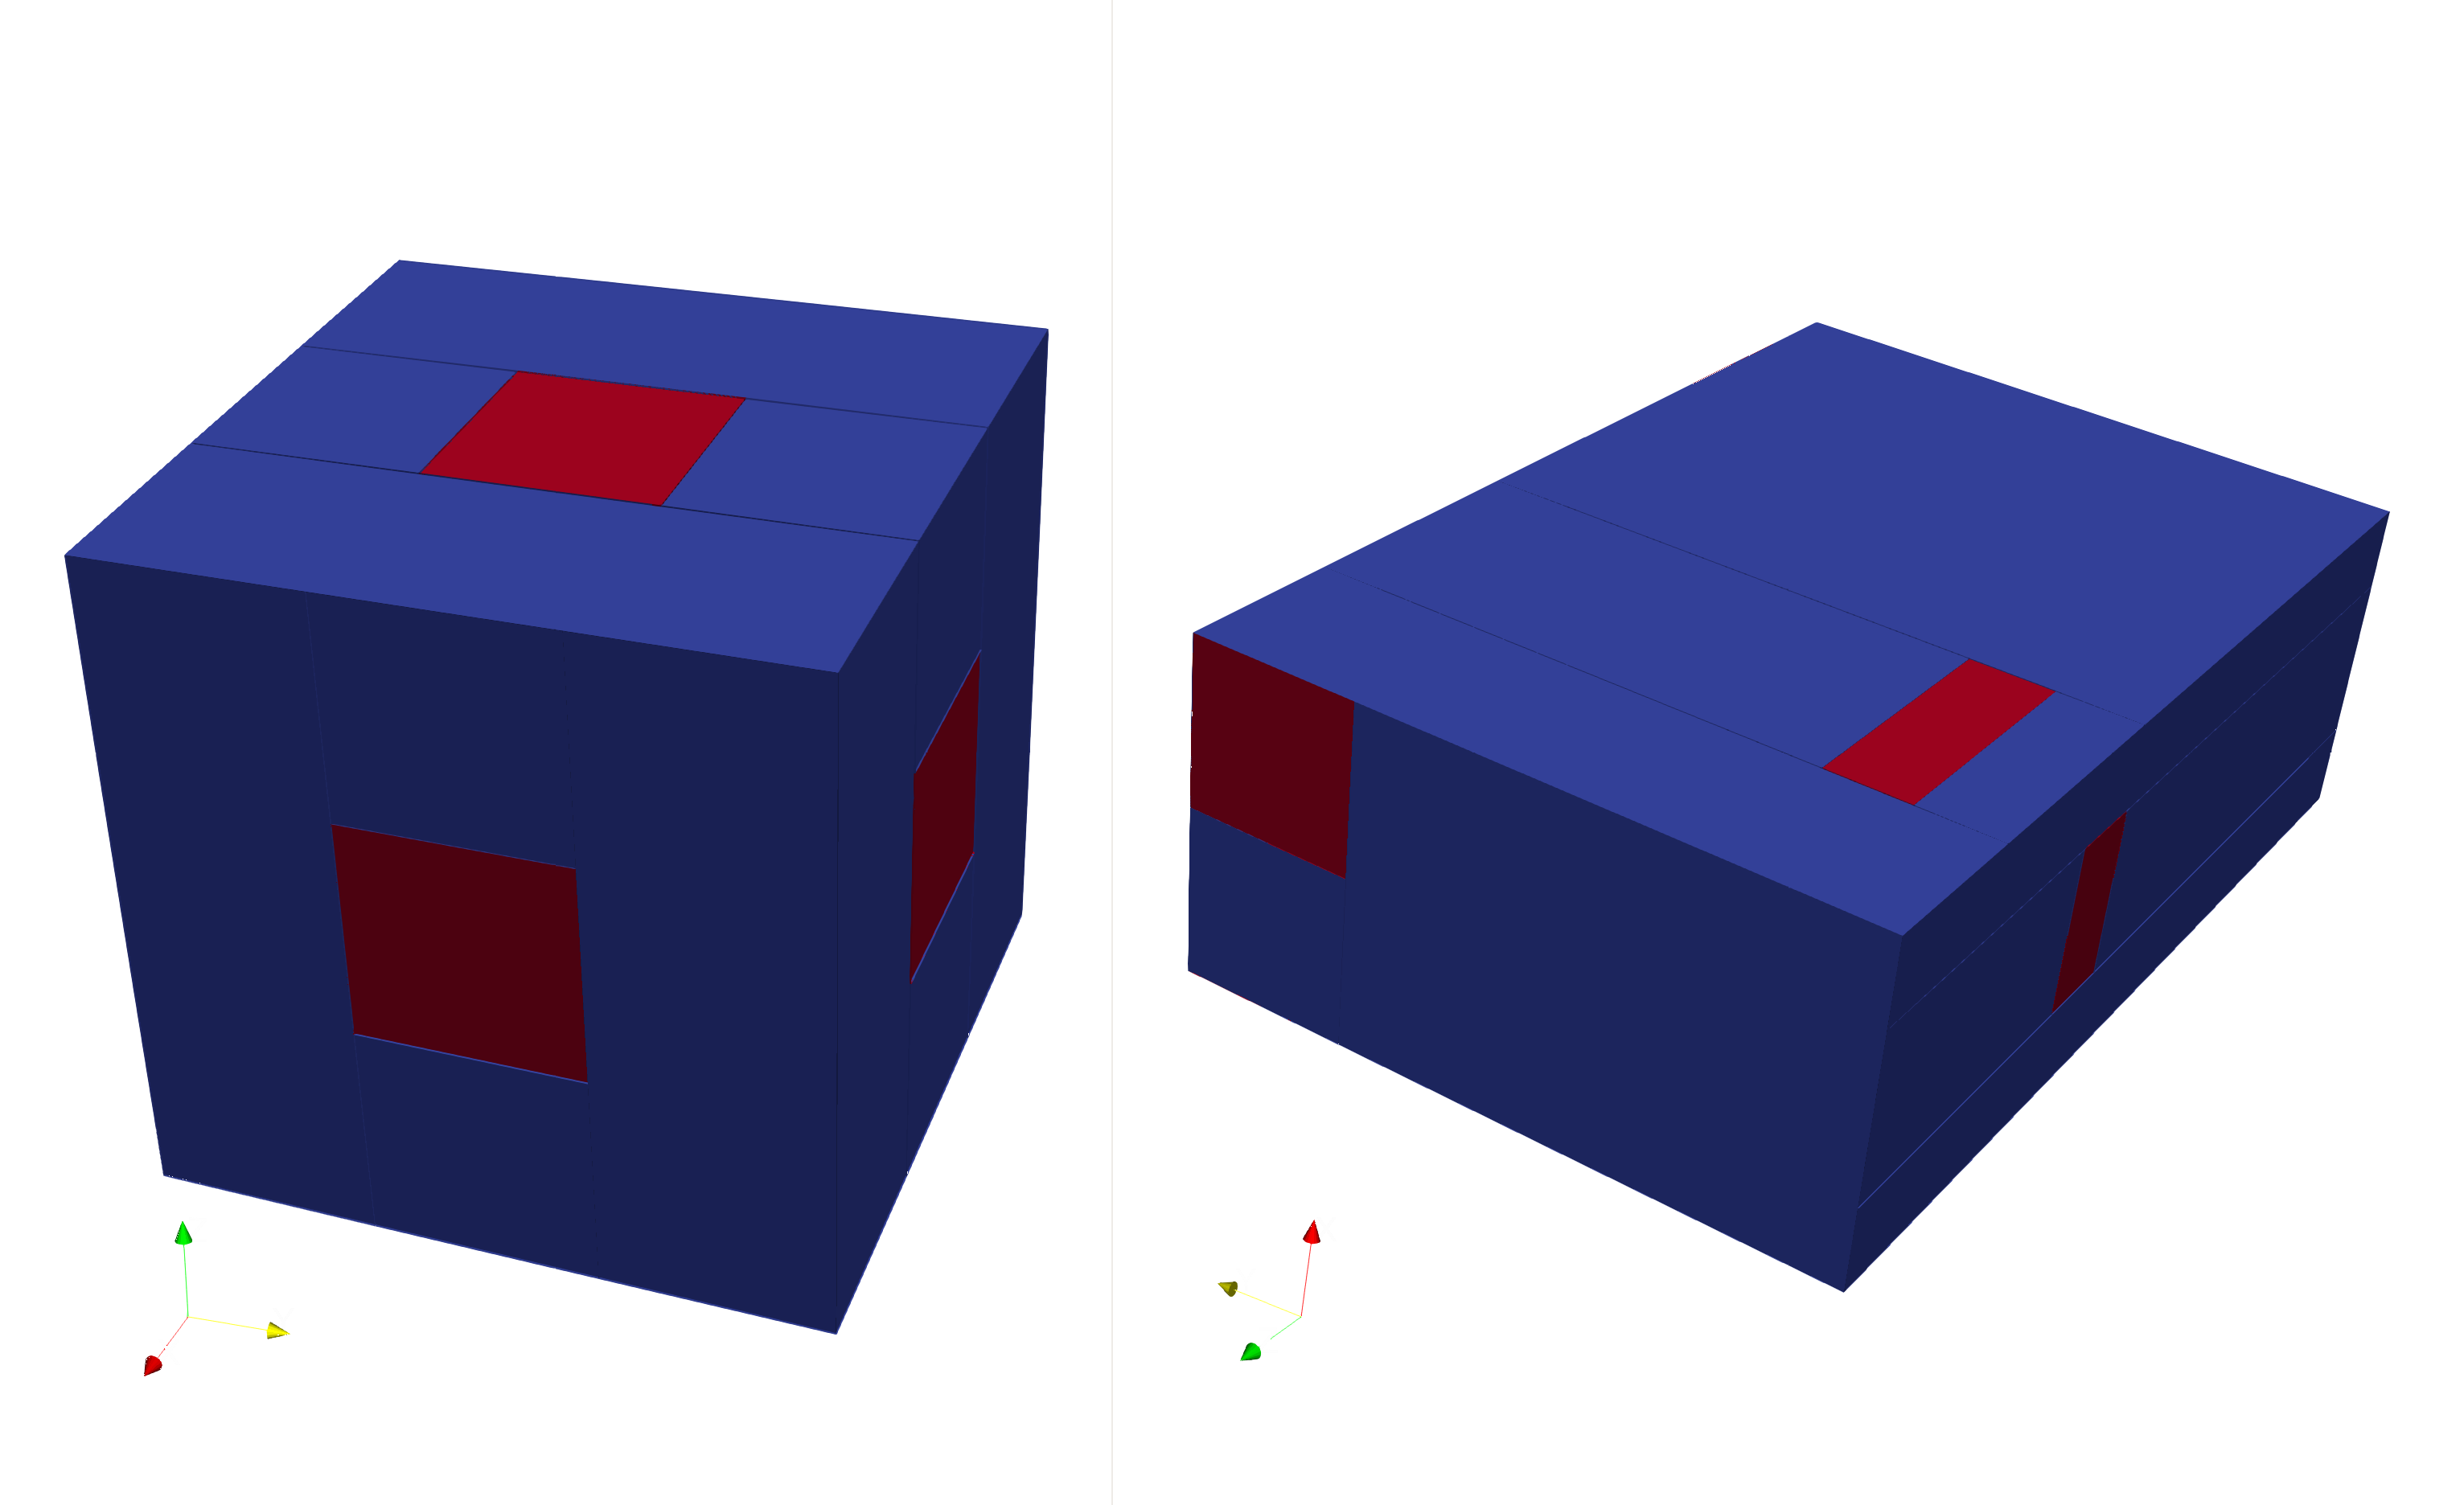
\includegraphics[width=0.7\textwidth]{cube_oid_ks_prop}
    \caption{Cube and cuboid for $k_{s}$ propagation test. Blue means
$k_{s} = 0.1$ and red equals $k_{s} =1.0$.}
    \label{fig:cube_oid_ks_prop}
\end{figure}

\paragraph{Overset cube}
The highjacked subroutine for the wall distance calculation takes a slightly
different path when overset meshes are used. To test it, the cube mesh from
before was repurposed. It was extendend with a coarse Cartesian  background
grid.  ADflow uses the \textit{implicit hole cutting scheme} to decide by itself
how to interpolate between those grids. As this was failing with the initial
grid, it has been refined slightly.

\subsection{Grid Convergence}

TBD

\subsection{Comparisons}
It is necessary to compare the SA rough implementation against theory and
experiments. As it is hard to get experimental data, the \textit{flat plat a
zero incidence} test case has been chosen for all comparisons. NASA maintains a
website called \textit{turbulence modeling resource} \cite{rumsey_flat}. There,
various formulations for different turbulence models may be found. Additionally
it provides testcases, grids and validation data. The following grid-family with
its corresponding boundary conditions was sourced from there (figure
\ref{fig:plate_bc}). Table \ref{tab:plate_sizes} lists the different mesh sizes.

\begin{figure}[H] \centering
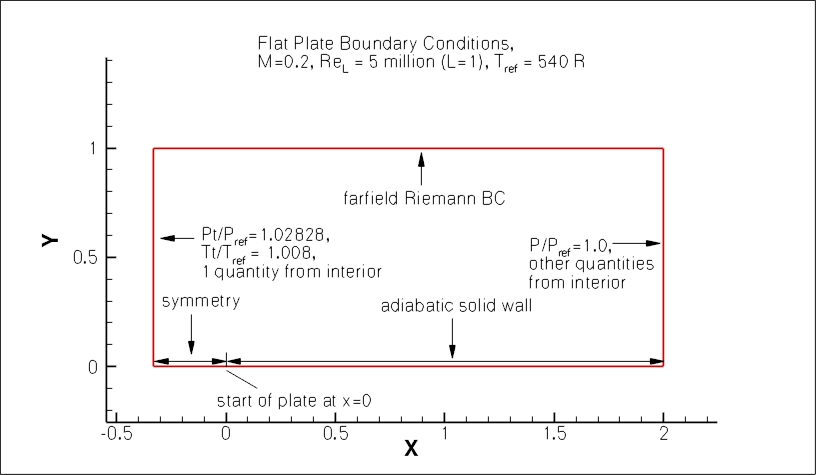
\includegraphics[width=0.7\textwidth]{plate_bc}
    \caption{Boundary conditions and test case overview \cite{rumsey_flat}.}
    \label{fig:plate_bc}
\end{figure}

\begin{table}[H]
  \centering
  \begin{tabular}{c r r}
    Identifier      & \# of nodes   & \# of cells \\
    \toprule
    L4              & 1'800         & 816 \\
    L3              & 6'860         & 3'264 \\
    L2              & 26'772        & 13'056 \\
    L1              & 105'764       & 52'224 \\
    L0              & 420'420       & 208'896 \\

  \end{tabular}
  \caption{Mesh sizes used for testcases.}
  \label{tab:plate_sizes}
\end{table}

\noindent The following cases were set up.

\paragraph{Clean}
The NASA TMR website \cite{rumsey_flat} provides numercial data on the skin
friction coefficient ($c_{f}$) for a clean wall. The SA rough model with a
surface roughness of $k_{s} = 0$ should match.

\paragraph{SU2}
SU2 is an open source solver \cite{su2} that has allready implemented SA rough.
Therefore it was natural to compare both implementations.

\paragraph{Acharya et al.}
Acharya et al. did some experiments with flows of a flat plates over rough walls.


TBD!!!!

\section{Automated tests}
ADflow uses automated tests to make sure no changes are breaking existing
features. This concept is know as \textit{regression tests}. Those tests may be
run for multiple times a day and their goal is to catch mistakes. Thus it makes
sense to speed them up as fast as possible. Because of that, the testcases have
really coarse meshes and their solution is most likely not physical; but this
does not matter.

As ADflow allready has some cases, it was easy to adapt and modify some of them
for the SA rough modification. The following new cases were introduced:


\begin{table}[H]
  \centering
  \begingroup
  \renewcommand{\arraystretch}{1.5} % adjust vertical spacing
  \begin{tabularx}{\textwidth}{lX}
    Test-Name                                     & Comment \\
    \toprule
    \texttt{TestAdjoint\_5\_Rough\_SA\_wing}      & 3D mesh of a wing whose
    surface is totally rough ($k_{s} = 0.001$).\\

    $\rightarrow$\texttt{rest\_residuals}        & Make sure ADflow converges to
    the same solution as a pre-trained reference file.\\

    $\rightarrow$ \texttt{rest\_adjont} & Make sure the adjoint vectors converge
    to the same solution as a pre-trained reference file.\\

    \texttt{TestCmplxStep\_5\_Rough\_SA\_wing}    & Same test as before, but use
    complex step. \\

    $\rightarrow$ \texttt{cmplx\_test\_aero\_dvs} & Make sure trained adjoint
    values from before are consistent with complex step (only aerodynamic design
    variables).\\

    $\rightarrow$\texttt{cmplx\_test\_geom\_dvs} & Make sure trained adjoint
    values from before are consistent with complex step (only geometric design
    variables).\\

    \midrule

    \texttt{TestFunctionals\_9\_Rough\_SA\_wing} & 3D mesh of a wing whose
    surface is totally rough ($k_{s} = 0.001$).\\

    $\rightarrow$\texttt{rest\_residuals}        & Make sure ADflow converges to
    the same solution as a pre-trained reference file.\\

    $\rightarrow$\texttt{rest\_restart\_read}    & Make sure restarts are possible.\\

    $\rightarrow$\texttt{rest\_functions}        & Make sure function values
    ($C_{l}$, $C_{d}$, etc.) are the same as a pre-trained reference file.\\

    $\rightarrow$\texttt{test\_forces\_and\_tractions} & Make sure tractions and
    forces are the same as a pre-trained reference file.\\

    $\rightarrow$\texttt{test\_jac\_vec\_prod\_fwd} & Make sure partial
    derivatives calculated using the forward mode are consistent with reference
    file. \\

    $\rightarrow$\texttt{test\_jac\_vec\_prod\_bwd} & Make sure partial
    derivatives calculated using the backwards mode are consistent with reference
    file. \\

    $\rightarrow$\texttt{test\_dot\_products} & Make sure the forward and
    backwards Algorithmic Differentiation is consistent using the dot-product test. \\

    \midrule

    \texttt{TestFunctionals\_10\_Rough\_SA\_wing} & Same tests as in
    \texttt{TestFunctionals\_9\_Rough\_SA\_wing}, but the reference file is from a
    previous testcase. This should make sure SA rough with $k_{s} = 0$ behaves like
    the standard SA model. \\

  \bottomrule

  \end{tabularx}
  \endgroup
  \caption{Mesh sizes used for testcases.}
  \label{tab:plate_sizes}
\end{table}



    \chapter{Results}
    \section{Roughness propagation}
As described in section \ref{subsec:roughness_prop}, three different test cases
were setup to verify the propagation of the surface roughness values to the
correct volume cells.

\subsubsection{Cube}
This test was designed to make sure the propagation is sound. Figure
\ref{fig:cube_ks_prop} shows the surface cube with the rough patch in the middle
of each face. The volume mesh is sliced in two axis and the propagation of the
roughness values can be seen.

\begin{figure}[H] \centering
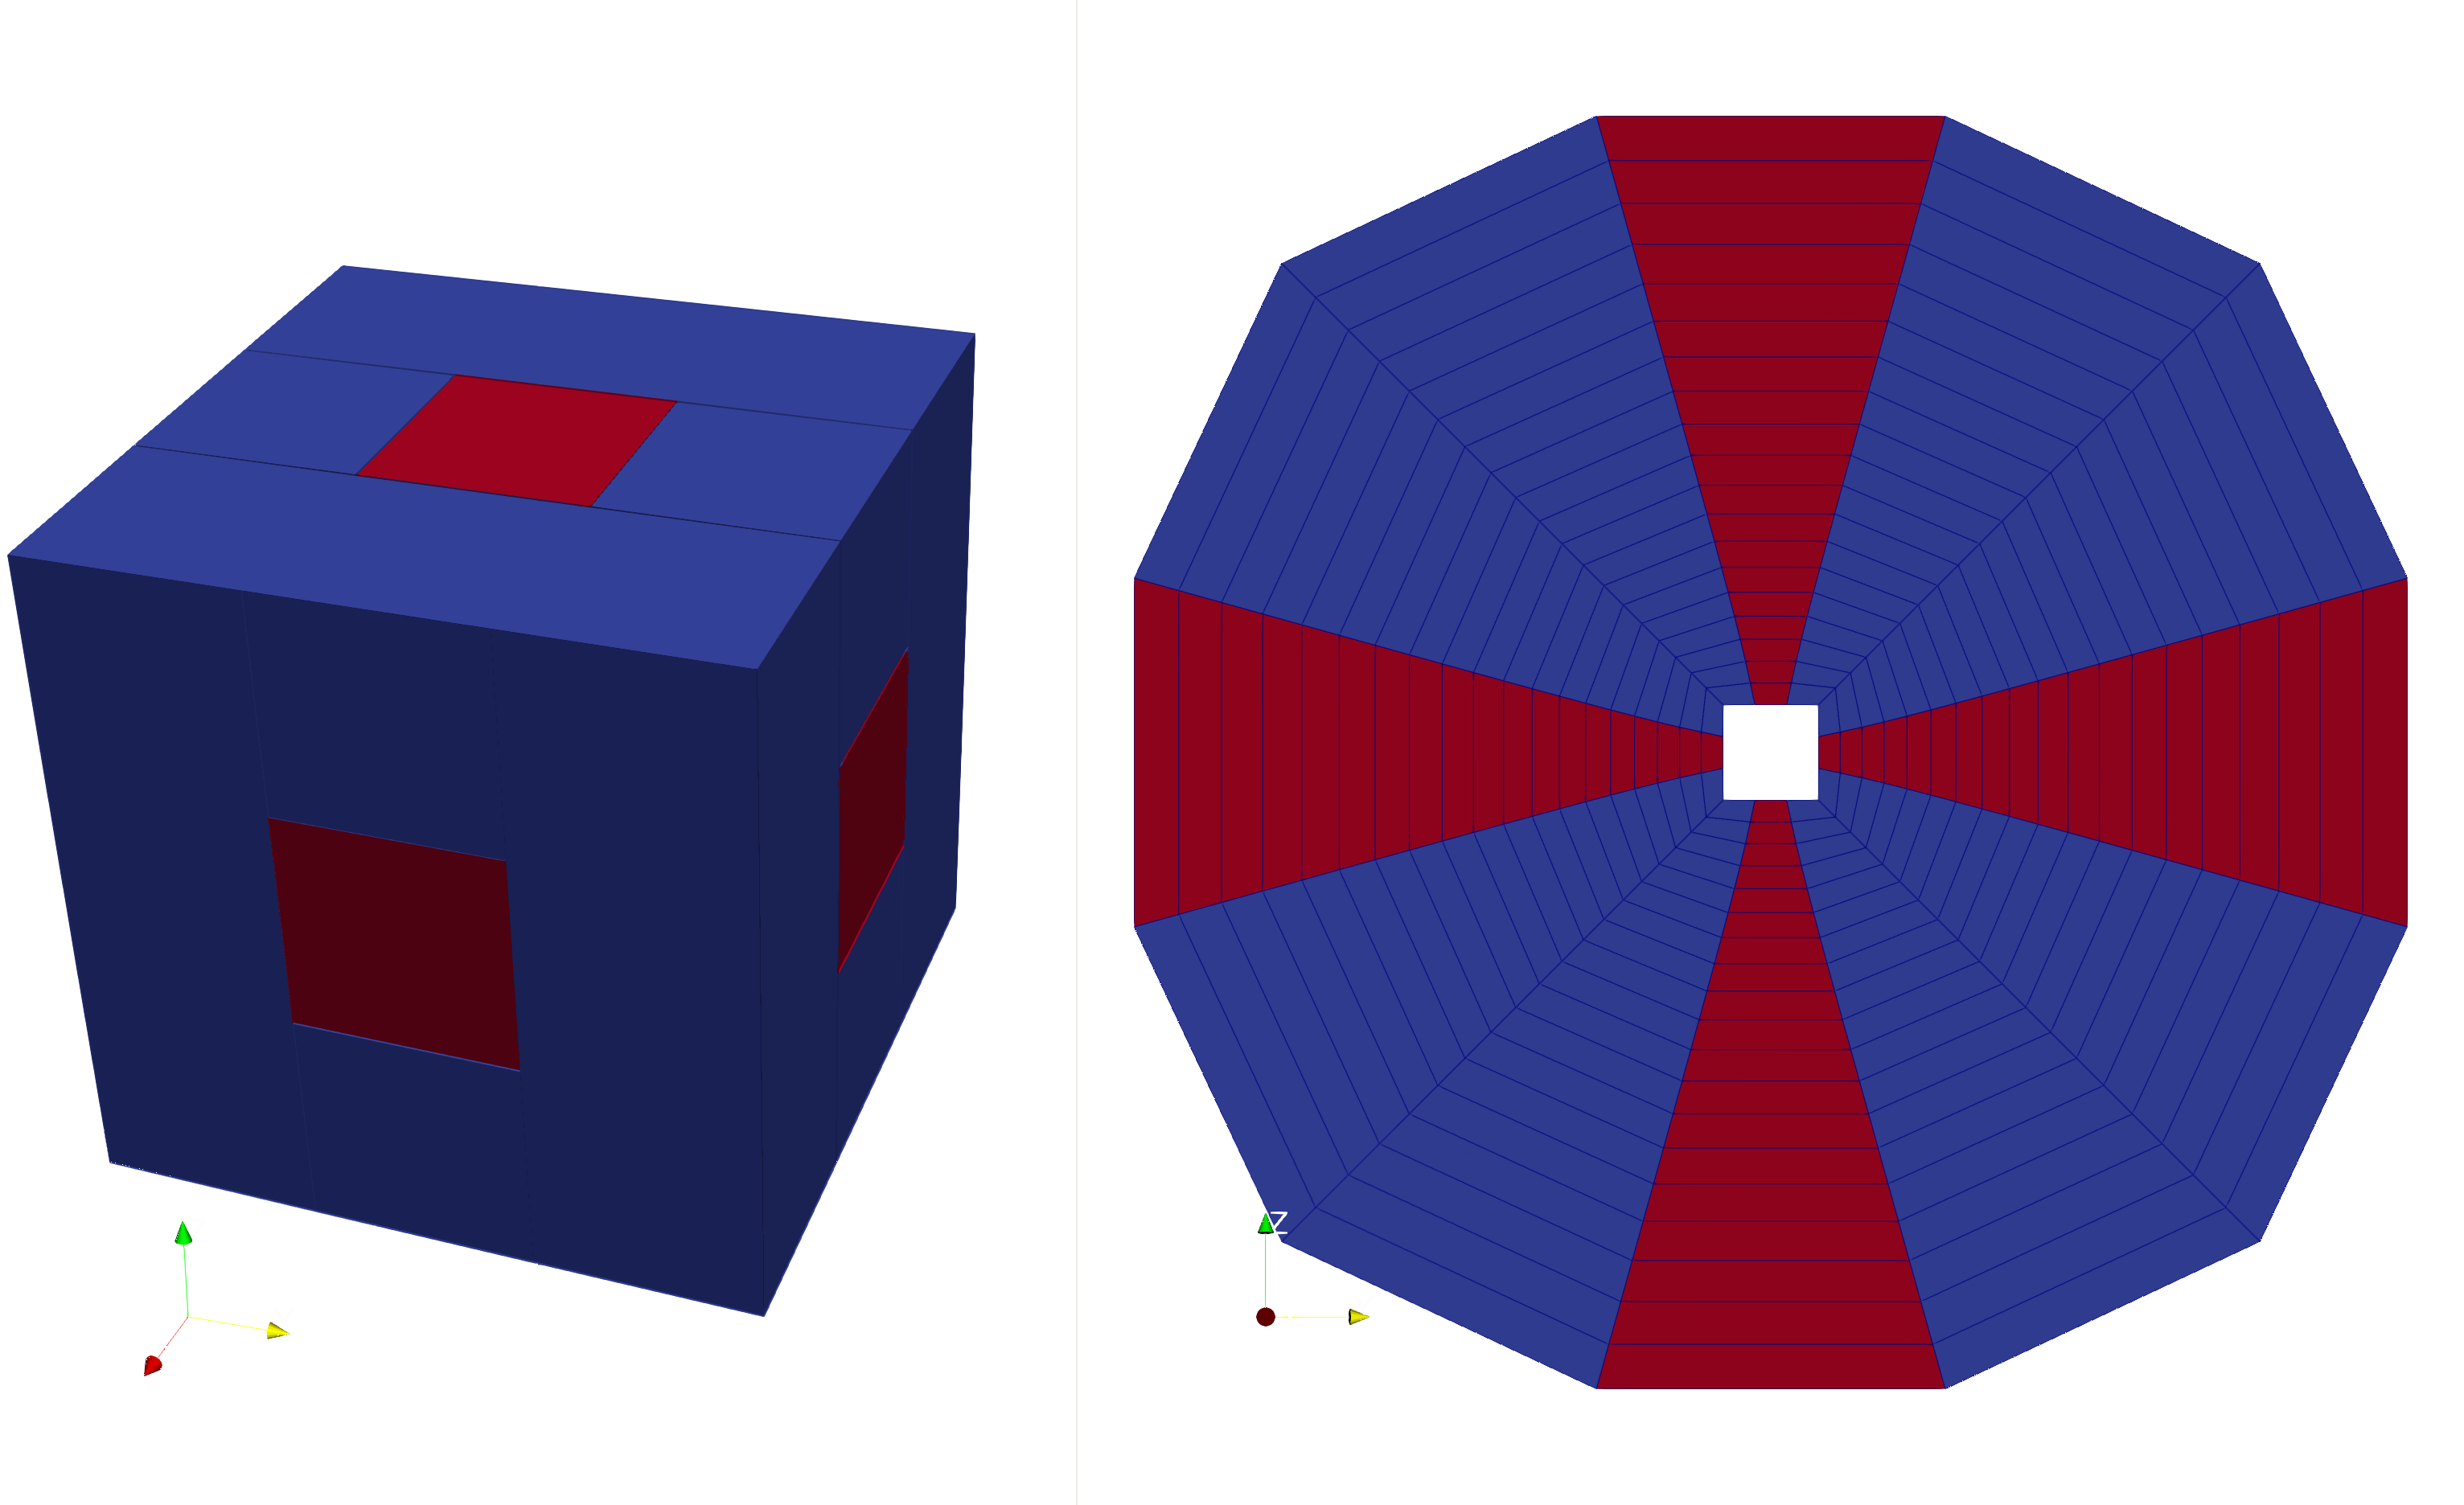
\includegraphics[width=0.5\textwidth]{cube_ks_prop.png}
    \caption{Cube with propagated roughness values. Red equals
$k_{s} = 1.0$ and blue $k_{s} = 0.1$.}
    \label{fig:cube_ks_prop}
\end{figure}

\subsubsection{Overset cube}
Similar to the previous test, it is used to show that the roughness values are
propagated correctly for  overset meshes. As described in section
\ref{subsec:roughness_prop}, it was necessary to refine the mesh a bit. This was
needed as the \textit{implicit hole cutting} would fail otherwise. In figure
\ref{fig:cube_overset_ks_prop}, the two overlapping meshes with the correctly
propagated roughness values is shown.

\begin{figure}[H] \centering
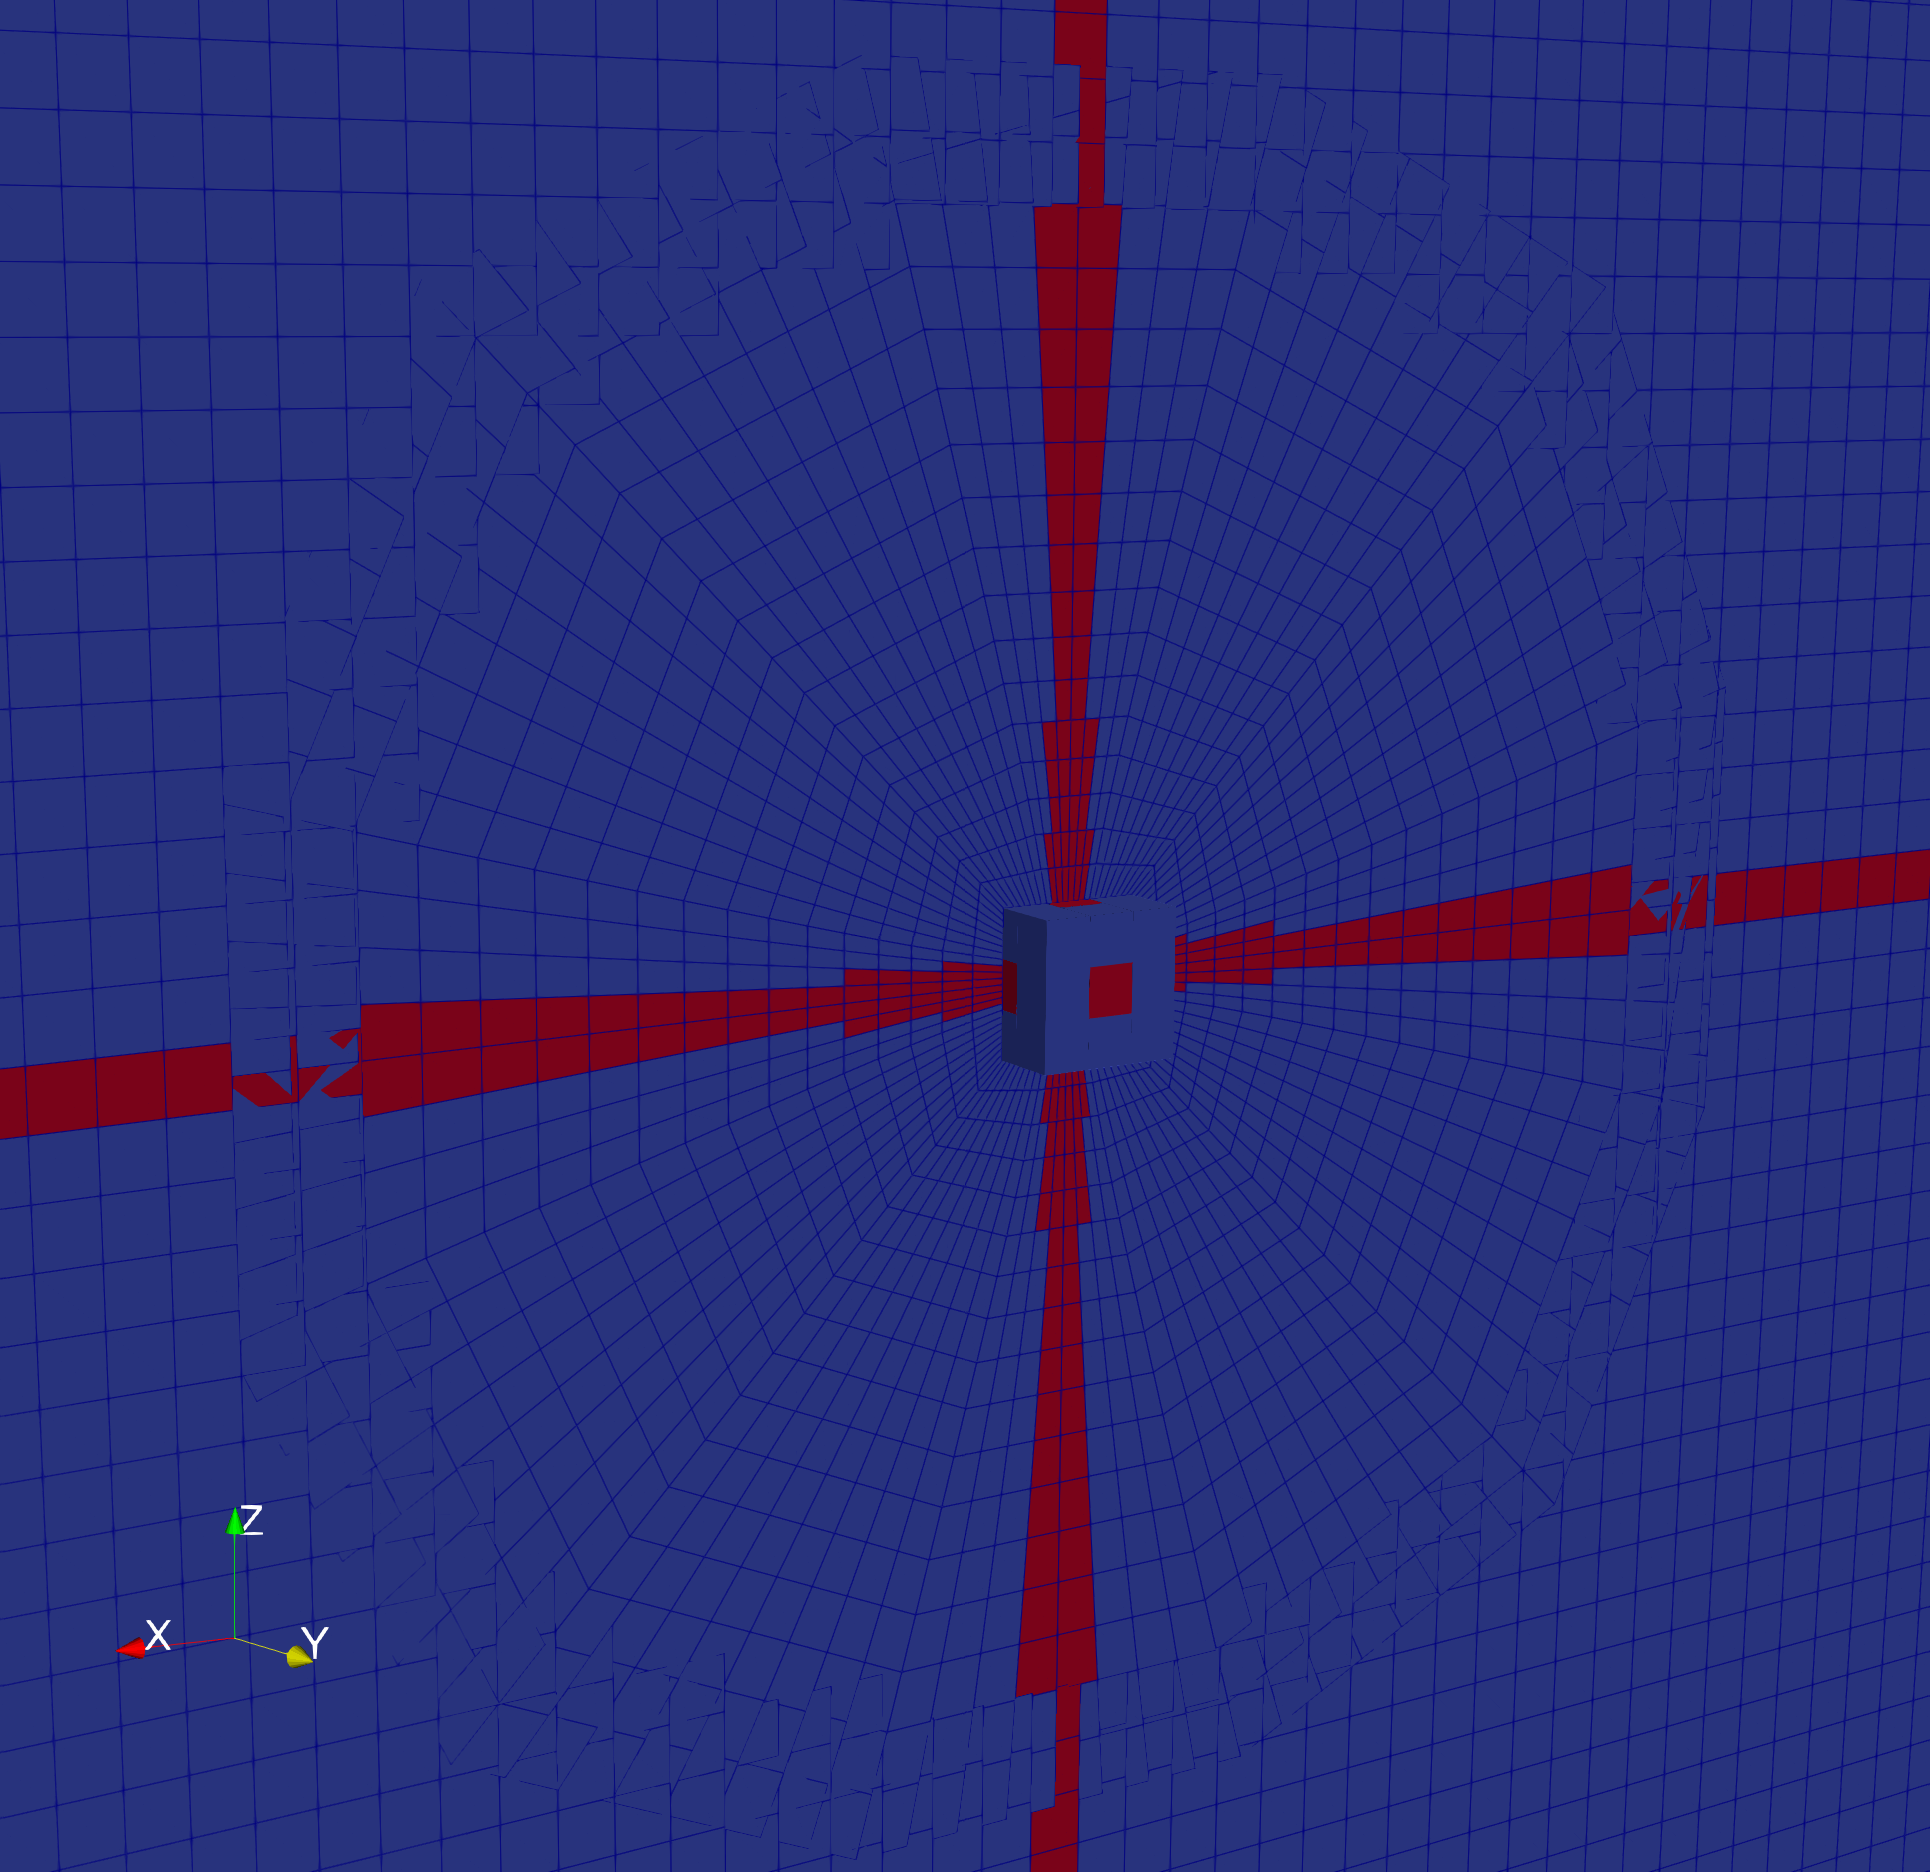
\includegraphics[width=0.5\textwidth]{cube_overset_ks_prop.png}
    \caption{Overset cube with propagated roughness values. Red equals
$k_{s} = 1.0$ and blue $k_{s} = 0.1$.}
    \label{fig:cube_overset_ks_prop}
\end{figure}

\subsubsection{Cuboid}
As described in section \ref{subsec:roughness_prop}, this 6 test cases were
designed to catch errors in the correlation of the surface cell to the global
cell index (\texttt{gID}). As such, no figures have been generated. But the
author is happy report that all tests have passed.

\section{Flap plate at zero incidence}

\subsubsection{Grid Convergence}
In figure \ref{fig:gc_rumsey_comp}, the grid convergence for various roughness
values is shown.  Additionally, grid convergence data for two different solvers
from \cite{rumsey_flat} is available for the skin friction coefficient. For
ADflow, the expected convergence rate is 2. When computing the actual ratio using equation
\ref{eq:conv_rate}, one gets a ratio of approximately 1. This is less than
expected and will be investigated further.

\begin{figure}[H] \centering
  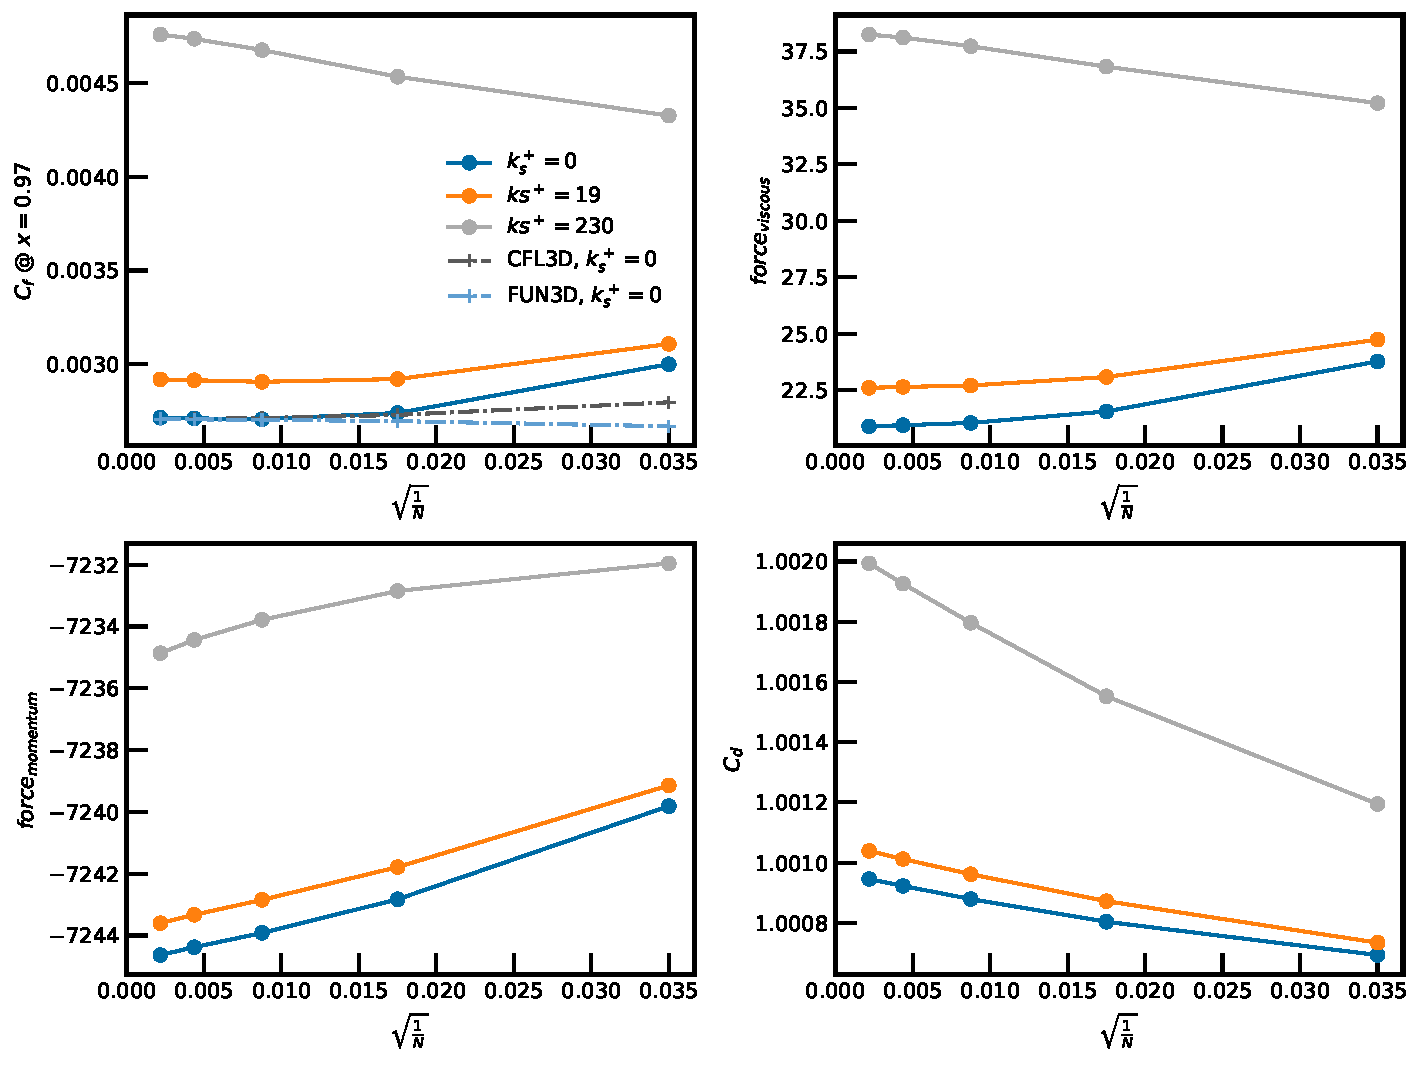
\includegraphics[width=0.9\textwidth]{comp/gc_rumsey_comp}
    \caption{Grid convergence for various roughness values. The skin friction
coefficient is overlayed with data from \cite{rumsey_flat}.}
    \label{fig:gc_rumsey_comp}
\end{figure}


\subsubsection{Clean}
In figure \ref{fig:cf_clean}, the skin friction coefficient over the flat plate
for a roughness value of $k_{s} = 0$ (clean) is shown. It is compared against
theory and data from the NASA TMR website \cite{rumsey_flat}. When looking
closely, ADflow and CFL3D agree well, but the theory is slightly off. The
agreement of both solvers indicates that the SA implementation is done correctly
(for a clean surface) in ADflow. The offset to theory probably means that the SA
model is not completely accurate in predicting the skin friction coefficient of
a flat plate.  It is unclear what the dip of the skin friction at the beginning
of the plate is. It may be explained as some kind of ``numerical'' transition. It
can be observed in other plots as well, but only for ADflow.

\begin{figure}[H] \centering
  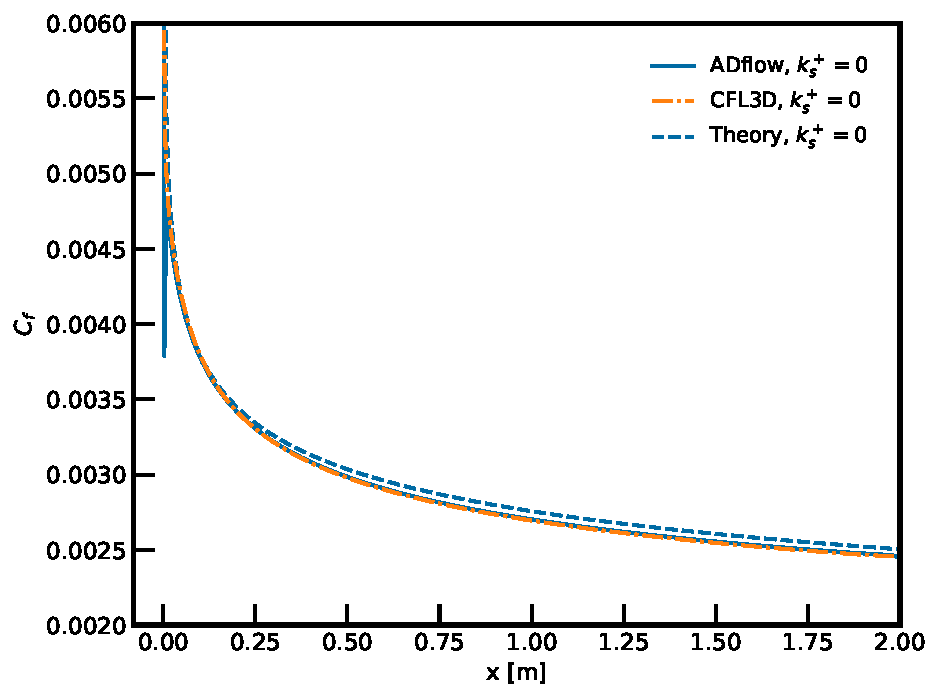
\includegraphics[width=0.6\textwidth]{comp/cf_clean}
    \caption{Skin friction coefficient for a roughness value of $k_{s} = 0$
      compared against theory and data from \cite{rumsey_flat}.}
    \label{fig:cf_clean}
\end{figure}

\noindent In figure \ref{fig:vp_clean}, the velocity profile at different
positions on the flat plate is plotted. It is compared against theory and
reference data from CFL3D. All curves agree well.
\begin{figure}[H] \centering
  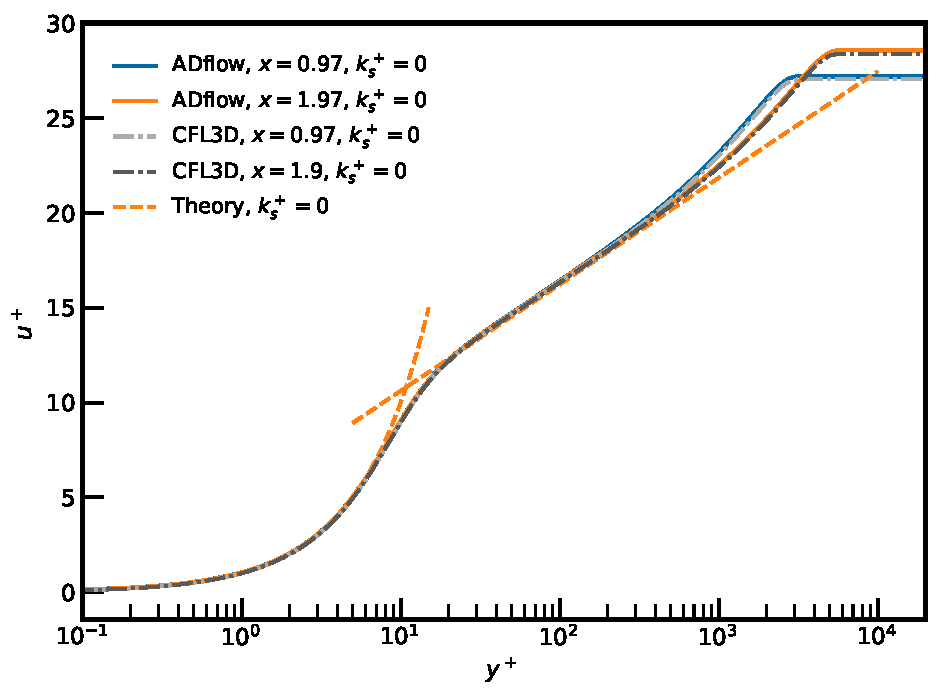
\includegraphics[width=0.6\textwidth]{comp/vp_clean}
    \caption{Velocity profile for a roughness value of $k_{s} = 0$ compared
      against theory and  data from \cite{rumsey_flat}.}
    \label{fig:vp_clean}
\end{figure}

\subsubsection{Blanchard}
In figure \ref{fig:cf_blanchard}, the skin friction coefficient for the clean
case and a roughness value of $k_{s}^{+} = 150$ is plotted. The clean case is
compared against theory and the rough against experimental data from Blanchard's
PhD thesis. But (as described in section \ref{subsec:flat_plate_exp}), the data
has been extracted from a different source \cite{sa_rough}. The theory and clean
case agree well, but the rough case does not. The ``numerical'' transition is
more obvious for the clean case. It also exists for the rough case, but is
seemingly inverted.

\begin{figure}[H] \centering
  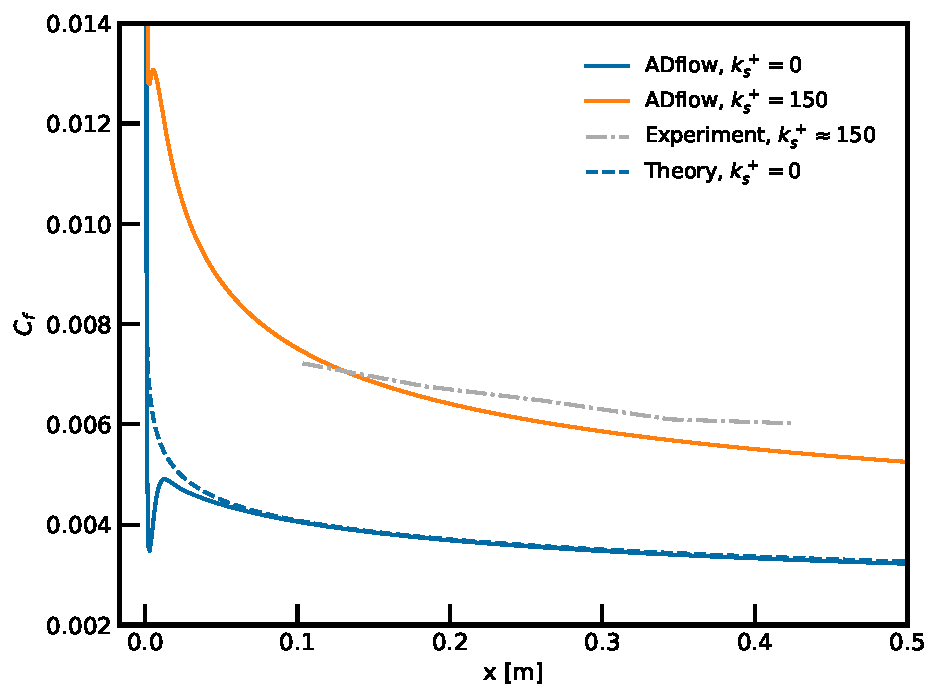
\includegraphics[width=0.6\textwidth]{comp/cf_blanchard}
    \caption{Skin friction coefficient for various roughness values compared
      against data from \cite{sa_rough}.}
    \label{fig:cf_blanchard}
\end{figure}


\subsubsection{Acharya et al.}
In figure \ref{fig:cf_acharya}, the skin friction coefficient for various
roughness values are plotted against theory and two experiments from
\cite{Acharya1986}. As before, the theory and clean case agree well. But the
rough cases do not. First of all, the skin friction coefficient is
under-predicted by ADflow. Coincidentally, the simulation for case two aligns
with case one. When ignoring the offset, one can conclude that at least the
predicted shape matches. The two curves do not agree at the beginning, but this
may be explained through transitional effects as the SA model is fully
turbulent. The ``numerical'' transition is again observable at the beginning of
the plate.

\begin{figure}[H] \centering
  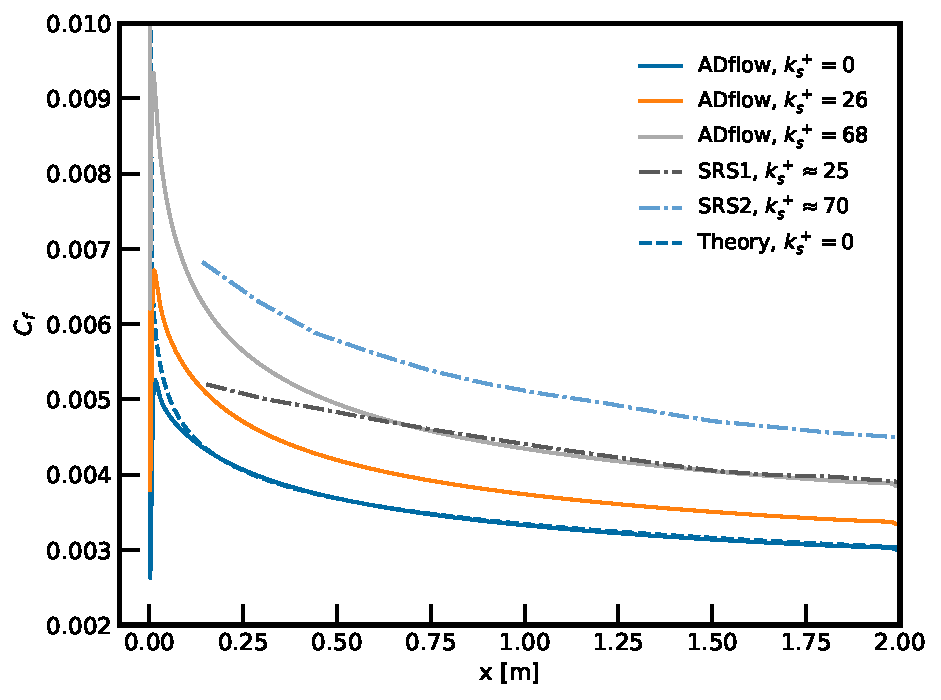
\includegraphics[width=0.6\textwidth]{comp/cf_acharya}
    \caption{Skin friction coefficient for various roughness values compared
      against theory and experimental data from \cite{Acharya1986}.}
    \label{fig:cf_acharya}
\end{figure}

\noindent In figure \ref{fig:vp_acharya}, the velocity profile for various
roughness values is plotted against theory and experimental data. Theory does
agree well for the clean case, but there is a big offset for the rough case.
ADflow values are not shifted enough. This indicates an underprediction of the
roughness effects which is consistent with the underprediction of the skin
friction coefficient. When looking at the experimental data, one can also
observe a slight underprediction. But this is explainable through the use of
mean values measured. This means, this curve also includes contributions from
places where the boundary layer has not fully developed.

\begin{figure}[H] \centering
  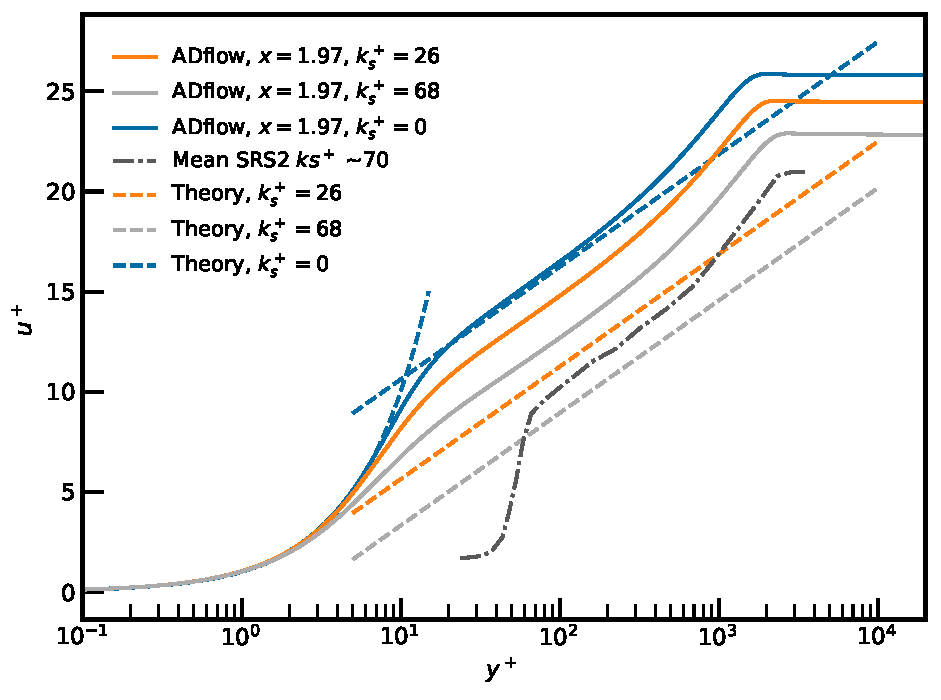
\includegraphics[width=0.6\textwidth]{comp/vp_acharya}
    \caption{Velocity profile for various roughness values compared
      against theory and experimental data from \cite{Acharya1986}.}
    \label{fig:vp_acharya}
\end{figure}



\subsubsection{SU2}
To validate the implementation itself, the skin friction coefficient for various
roughness values is plotted against data from SU2. For the clean case, both
solvers agree well. But for the rough cases, one can observe the same offset as
seen before. For ADflow, the ``numerical'' transition can be seen clearly at the
beginning. For SU2, it is obscured, but the author reports that it does not
exist.

\begin{figure}[H] \centering
  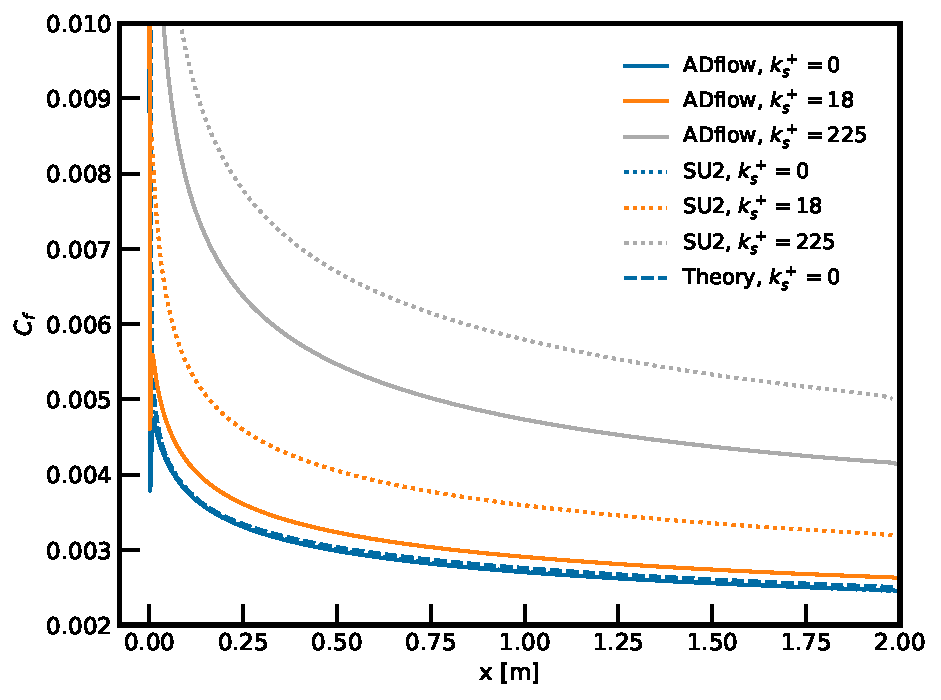
\includegraphics[width=0.6\textwidth]{comp/cf_rumsey_comp}
    \caption{Skin friction coefficient for various roughness values compared
      against theory and SU2.}
    \label{fig:cf_rumsey_comp}
\end{figure}

\noindent In figure, \ref{fig:vp_rumsey_comp}, the velocity profile for
different roughness values is shown. For the clean case, both solvers agree well
with theory. SU2 does also agree well for the rough cases although having a
slight offset. For ADflow, the same shift compared to SU2 and theory is
observable.

\begin{figure}[H] \centering
  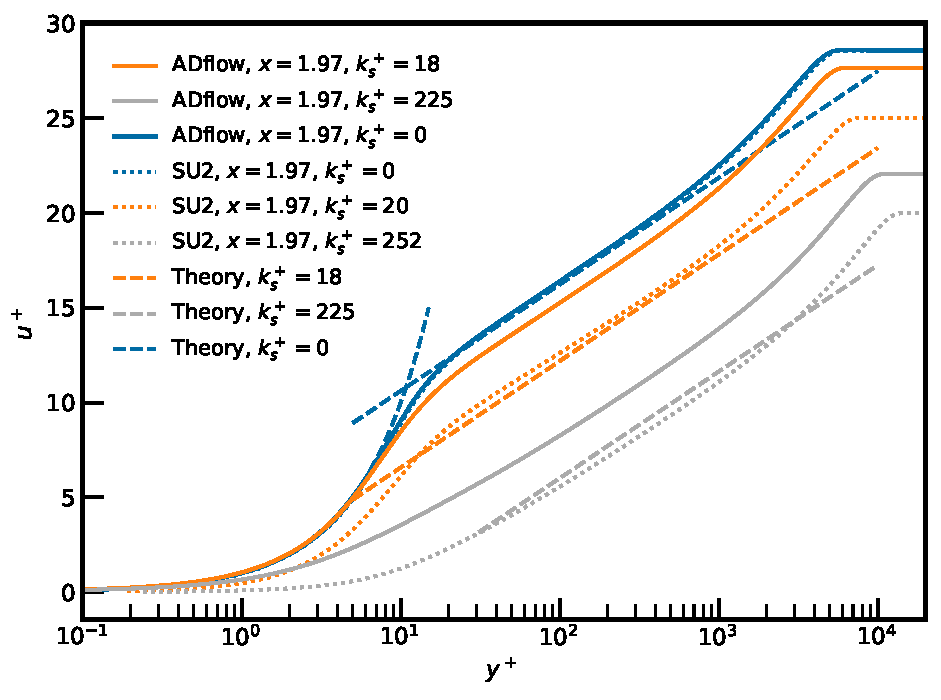
\includegraphics[width=0.6\textwidth]{comp/vp_rumsey_comp}
    \caption{Velocity profile for various roughness values compared
      against theory and SU2.}
    \label{fig:vp_rumsey_comp}
\end{figure}

\subsection{Offset}
As has been shown in the last section, the SA rough implementation in ADflow is
somehow not correct. It is observable that the predicted shapes of the curves are
correct, but they seem to be offset compared to experiments and SU2. At the time
of writing it is not clear what is causing this and will be investigated
further.

\section{Automated tests} Reporting the results of the automated tests is
easiest done in tabular form. Take a look at table \ref{tab:tests_results}.


\begingroup
\renewcommand{\arraystretch}{1.5} % adjust vertical spacing
\begin{xltabular}{\textwidth}{lX}
    \toprule
    Test-Name                                     & Comment \\
    \toprule
    \endhead
    \texttt{TestAdjoint\_5\_Rough\_SA\_wing}      & \\

    $\rightarrow$ \texttt{rest\_residuals}        & Passes to an absolute and
    relative tolerance of \num{1e-10}. \\

    $\rightarrow$ \texttt{rest\_adjoint}           & Passes to an absolute and
    relative tolerance of \num{1e-10}. \\

    \midrule

    \texttt{TestCmplxStep\_5\_Rough\_SA\_wing}    & \\

    $\rightarrow$ \texttt{cmplx\_test\_aero\_dvs} & Passes to an absolute
tolerance of \num{5e-10} and a relative tolerance of \num{1e-8}. \\

    $\rightarrow$ \texttt{cmplx\_test\_geom\_dvs}& Fails with an absolute and relative
    tolerance of \num{5e-9} as follows:\\

    &\begingroup
    \renewcommand{\arraystretch}{1.0} % adjust vertical spacing
    \begin{tabular}{l l r r}
      Functional & design var. & abs. tol.      & rel. tol. \\
      \toprule
      $C_{l}$    & span        & \num{1.64e-8}  & \num{3.77e-7} \\
      $C_{d}$    & span        & \num{9.39e-9}  & \num{6.44e-6} \\
      $C_{mz}$   & span        & \num{2.62e-8}  & \num{4.10e-7} \\
      lift       & span        & \num{6.67e-3}  & \num{3.77e-7} \\
      drag       & span        & \num{4.42e-4}  & \num{4.73e-7} \\
      $C_{l}$    & twist       & \num{7.21e-9}  & \num{2.92e-7} \\
      $C_{l}$    & shape       & \num{2.29e-7}  & \num{3.45e-4} \\

    \end{tabular}
    \endgroup

    \\

    &Please note some design variables are neglected as it does not improve the
    overall picture.

    \\

    \midrule

    \texttt{TestFunctionals\_9\_Rough\_SA\_wing} & \\

    $\rightarrow$ \texttt{rest\_residuals}        & Passes to an absolute and
    relative tolerance of \num{1e-10}. \\

    $\rightarrow$ \texttt{rest\_restart\_read}    & Passes to an absolute and
    relative tolerance of \num{1e-10}. \\

    $\rightarrow$ \texttt{rest\_functions}        & Passes to an absolute and
    relative tolerance of \num{1e-9}. \\

    $\rightarrow$ \texttt{test\_forces\_and\_tractions} & Passes to an absolute and
    relative tolerance of \num{1e-10}. \\

    $\rightarrow$ \texttt{test\_jac\_vec\_prod\_fwd} & Passes to an absolute and
    relative tolerance of \num{5e-9}. \\

    $\rightarrow$ \texttt{test\_jac\_vec\_prod\_bwd} & Passes to an absolute and
    relative tolerance of \num{1e-10}. \\

    $\rightarrow$ \texttt{test\_dot\_products} & Passes to an absolute and
    relative tolerance of \num{1e-10}. \\

    \midrule

    \texttt{TestFunctionals\_10\_Rough\_SA\_rans\_tut\_wing} & All tests pass.
    The tolerances are the same as for
    \texttt{TestFunctionals\_9\_Rough\_SA\_wing} listed above.\\

  \bottomrule

  \caption{Results from automated tests.}
  \label{tab:tests_results}
\end{xltabular}
\endgroup


\noindent All tests passing except for the geometric design variables in
\texttt{TestCmplxStep\_5\_Rough\_SA\_wing} indicates that there might be
something wrong with the geometric derivatives. It is unclear what is causing
this and will be investigated further. Although it is important to point out the
size of the relative error of \num{1e-7} is already quite small. For
comparison, the  \textit{finite differences} approach would only yield such
accurate gradients when finding the perfect step length, which is not to be
expected. Nevertheless, a relative tolerance of less than \num{1e-8} should be
achievable with the methods employed.



    \chapter{Conclusion}
    During the course of this project, a modification to the Spalart Allmaras (SA)
turbulence model for rough walls has been implemented. The changes have been
proposed by Boeing and published by \cite{sa_rough}. The SA model is a
one-equation model that solves for the eddy viscosity. The distance to the wall
is used for the turbulence length scale. The modification for rough walls simply
changes this distance, meaning it shifts a virtual wall upwards. This increases
the height of the boundary layer which is the primary effect of roughness.

To modify the wall distance, the roughness value of the nearest surface cell is
needed. This might sound easy on first sight. But one has to keep in mind that
ADflow is a parallel code. This means the whole mesh is split across different
processors. Each processors has only access to mesh cells he owns. Thus the
roughness value of the nearest wall for the current cell might live on a
different processor and must be communicated across. Figuring out this
communication was challenging and error prone. To make sure it was implemented
correctly, testcases with cubes and cuboids were set up. Those tests would
either fail or look wrong when the communication was not implemented correctly.

To validate the modifications itself, test cases with rough walls were setup.
Those cases compare ADflow to experimental data, theory and the open source
Solver SU2. They could show that the rough modification with a surface roughness
of 0 would still be the same as the standard SA model. Unfortunately, they also
made it clear that current implementation has a bug where the skin friction
coefficient and the velocity profile are wrongly shifted for rough surfaces.
This means, the predicted shape looks right, but the predicted values are not.
It is unclear what is causing this. It will be investigated in the future.

The before mentioned test cases also showed that the expected grid convergence
rate of 2 was not achieved. The real value lies more around 1. This will also be
investigated further.

Lastly, automated tests were setup to make sure future changes do not break
existing features. This concept is know as regression tests. In ADflow, the
automated tests are also mixed with unit tests which prove a new feature is
working. In this context, the gradients of the modified SA model was compared
against complex step. Unfortunately, they do not completely agree and are off by
a relative tolerance of \num{1e-7}. It is unclear what was causing this and will
be investigated further.

To conclude, a solid base was created. Although some bugs are still present that
need further work. Luckily, they do not affect an optimization in the following
sense: (1) The lower than expected grid convergence does not directly affect an
optimization. (2) The offset of the gradients is so small that an optimization
would still converge, maybe a bit slower. (3) The offset of the roughness
effects can be compensated with a higher than expected surface roughness value.
This is possible because the predicted shape of the roughness effects match.
And lastly, in optimization, it is more important to take effects of roughness
into account than accurately predicting those. After all, it is extremely
difficult to define a valid roughness value for e.g a soiled wind turbine blades
after 20 years of service.


    \printbibliography

\end{document}
